%TODO: add names of the models (gamodel mostly and adequade the params and stuff)
%\chapter{Metodologia Proposta}\label{chapter6}
%TODO: Add section about regions data, move it from the catalog data
%TODO: heat maps
%TODO: boxplot
%TODO: how to produce forecast
%TODO:  how to evaluate
%TODO: add paired test results
\section{Genoma Representation}
Each individual represents an earthquake risk model. It has a number of bins chose to fit the area of study and each bin has a probability value. The areas of study are: Kanto, Kansai, East Japan or Touhoku, see section~\ref{capitulo5}. To obtain the number of earthquakes by the value of the bin, we use the modified Poisson distribution~\cite{NumericalRecipes}.   
	
\begin{algorithm}
  \caption{Obtaining values between $[0,1)$ from the Poissonian curve.}
  \label{InversePoisson}
  \begin{algorithmic}
    \STATE Parameters $0 \leq x < 1, \mu \geq 0$
    \STATE $L \gets \exp{(-\mu)}, k \gets 0, prob \gets 1$
    \REPEAT 
    \STATE $\text{increment }k$
    \STATE $prob \gets prob*x$
    \UNTIL{$prob > L$}
    \RETURN $k$
  \end{algorithmic}
\end{algorithm}	

The scale chosen for the bins of each area were defined by taking into account that the resolution of a prevision model is inversely proportional to the size of the bin. That means that the smaller the bin scale, the higher is the resolution of this model. Also, we decided that each bin would have a scale depeding of the area. Once both Kansai and Kanto regions cover an area of 25 Km$^2$ the scale of theirs bins is set to 0.05 degress. Once they cover a smaller area, when compared with the areas of Touhoku and East Japan, we definided, for Touhoku and East Japan, a scale of the bin a little bigger, being 0.1.\\

To accelerate the development of the prototype we used the {\it Distributed Evolutionary Algorithms in Python} - DEAP \cite{DeRainville:2012:DPF:2330784.2330799}, a framework for Genetic Algorithms.
Its design seeks to make algorithms explicit and data structures transparent. \cite{DeRainville:2012:DPF:2330784.2330799}.\\

\section{Simple L-test Fitness Function}
We first intented to used the L-test, see~\ref{Ltest}, as fitness function. Once the main goal was to find if this fitness fuction would produce good results, we focus ours effort only in developing a application that would provides us fast results. Therefore, no study related with the GA paramerters and its values were made. We calculated the L-test the individuals and the one with the biggest value would be maintained into the next generation.\\

Once no effort was made to analyse the GA initial population and number of generations, we chose them by trial and error, until an acceptable convergency time were achieved.\\

We used all earthquake data available in Kanto, not taking into account the anual slices~\ref{capitulo5}.\\

\subsection{Crossover}
The results from the executions of the Simple L-test Fitness Function were obtained by using two crossover operators the Blend and the Two Points operators.\\

As defined in~\cite{takahashi2001crossover}, the Blend crossover is as follows:uinte forma:

\begin{enumerate}
  \item Choose two parents, $x^1$ e $x^2$, at random.
  \item A value for each element of the children $x^c_i$ of the next population is randomly chosen of the interval $[X^1_i, X^2_i]$ of the following distribuition:
\begin{center}
	\begin{equation}
	\begin{split}
		X^1_i = min(x^1_i,x^2_i) - \alpha d_i		\\
		X^2_i = max(x^1_i,x^2_i) + \alpha d_i 		\\
d_i = |x^1_i,x^2_i| \\
	\end{split}
	\end{equation}
\end{center}
where $x^1_i$ and $x^2_i$ are the $i$-th element of $x^1_i$ e $x^2_i$, respectively, and $\alpha$ is a positive parameter.
\end{enumerate}

Herrera, Lozano and Verdegay~\cite{herrera1998tackling} state that with an $\alpha$ = 0.5 there is balance between exploitation and exploration. Based on this, the value used for $\alpha$ was set to 0.5.\\

the Two Points crossover was used to compared the effect between different kinds of crossover operators. As it is defined by Goldeberg,~\cite{Goldberg:1989:GAS:534133}, it is considired a two-step operator. This crossover operator is an instance of the n-point crossover operator (where ${\it n} = 2$) which are a generalization of the simple crossover,~\cite{herrera1998tackling}.\\

The first step of the Two Points crossover is to choose two parents, at random. After that, each parent is splited into two parts, given a position k. This value is a number randomly chosen from a uniform distribuition, with the limits 1 to the maximum length of the individuals minus 1, $[1, {\it l} -1]$. The children then is generating by swapping the data from the parents.\\

\subsection{Mutation Operator}

The mutation operator chosen was the FlipBit. It swaps the bit value from each element and uses a value between $0$ to $1$ to decide if an idividual will be altered by the it~\cite{Goldberg:1989:GASac:534133}.
\subsection{Selection Operator}
For the selection operator we used the Simple Tournament and Elitism. The Simple Tournament was used to select individuals to participate on the reproduction, based on the fitness values they obtained. The elitism were used to impose that the best individual fromthe current generation would be part of the next generation, ensuring that the next generation has quality at least as good as the former one.\\

The parameters from the application with the Simple L-test are estão described in the next chart~\ref{GAParameters-Ltest}:\\

\begin{table}[!h]
  \begin{center}
  \begin{tabular}{|l|r|}
    \hline
    Population size & 500\\
   	Number of generations & 100\\
    Blend crossver $\alpha$ & 0.5\\
    Mutation FlipBit & 0.2\\
    Probability of Mutation(indpb) & 0.05 \\
    Tournament size & 3\\
    \hline    
  \end{tabular}
  \end{center}
  \caption{Used Parameters.}
  \label{GAParameters-Ltest}
\end{table}

\section{Time-slice Log-Likelihood Fitness Function}
After some analyses made on the last application, we realized that our model were overfitting with the data. Once this is not interesting, some changes were made.\\

First, we changed the fitness function from the L-test to the Log-likelihood value~\ref{log-fuction}. We also started using the the anual slices, described in the chapter~\ref{capitulo5} for the region of Kanto.\\


\subsection{Available Operators}
In this case, a wider experiment was made. We compared all operators from the DEAP framework and selected the group that achieve greater results.\\ 

\subsubsection{DEAP operators}

The parameters used in Time-slice Log-Likelihood are the ones from the chart~\ref{GAParameters-2}.\\

\begin{table}[!h]
  \begin{center}
  \begin{tabular}{|l|r|}
    \hline
    Popluation size & 500\\
    Numner of generations & 100\\
    Crossover operator & 0.9\\
    Mutation operator & 0.1\\
    \hline    
  \end{tabular}
  \end{center}
  \caption{Used parameters.}
  \label{GAParameters-2}
\end{table}

The operators from DEAP are described as follows. All descriptions were obatined from the DEAP framework webapge~\cite{webDeap}.\\

\paragraph{Crossover}
The operators used were: {\it One Point}, {\it Uniform}, {\it Two Points}, {\it Partially Matched}, {\it Ordered} and {\it Simulated Binary}.\\

\subparagraph{One Point}
It executes the one point crossover. Both parents are modified and the children have the same length as the parents.\\

\begin{table}[!h]
  \begin{center}
  \begin{tabular}{|l|r|}
    \hline
    Parameter (1) & An inidividual\\
    Parameter (2) & An inidividual\\
    Return & 2 modified individuals\\
    \hline    
  \end{tabular}
  \end{center}
  \caption{Parameters and return of the One Point crossover}
  \label{One Point}
\end{table}

\subparagraph{Uniform}
It executes the uniform crossover that modifies two parents. The elements are modified to a new value from an uniform distribuition according to a given probability, genneralt set to 0.5.\\

\begin{table}[!h]
  \begin{center}
  \begin{tabular}{|l|r|}
    \hline
    Parameter (1) & An inidividual\\
    Parameter (2) & An inidividual\\
    Parameter  (3) & A probabilty value\\
    Return & 2 modified individuals\\
    \hline    
  \end{tabular}
  \end{center}
  \caption{Parameters and return of the Uniform crossover}
  \label{Uniform}
\end{table}

\subparagraph{Partially Matched}
It executes on the two parents a partially matched crossover. The individuals are created by matching the index pais of the parents given a interval and then exchanging their values.\\

\begin{table}[!h]
  \begin{center}
  \begin{tabular}{|l|r|}
    \hline
    Parameter (1) & An inidividual\\
    Parameter (2) & An inidividual\\
    Return & 2 modified individuals\\
    \hline    
  \end{tabular}
  \end{center}
  \caption{Parameters and return of the  Partially Matched crossover}
  \label{Partially Matched}
\end{table}

\subparagraph{Uniform and Partially Matched}
It executes a combination of the Uniform and Partially Matched crossovers. In follows the same behavior as the last one but index matching is done randomly as in the Uniform crossover.\\

\begin{table}[!h]
  \begin{center}
  \begin{tabular}{|l|r|}
    \hline
    Parameter (1) & An inidividual\\
    Parameter (2) & An inidividual\\
    Return & 2 modified individuals\\
    \hline    
  \end{tabular}
  \end{center}
  \caption{Parameters and return of the Uniform and Partialy Matched crossover}
  \label{Uniform and Partially Matched}
\end{table}

\subparagraph{Ordered}
Executes an ordered crossover on the two parents. It select a interval of indexes from a parent and swaps the values from this intervals with the values from the other parent the the same interval of indexes, in order.\\

\begin{table}[!h]
  \begin{center}
  \begin{tabular}{|l|r|}
    \hline
    Parameter (1) & An inidividual\\
    Parameter (2) & An inidividual\\
    Return & 2 modified individuals\\
    \hline    
  \end{tabular}
  \end{center}
  \caption{Parameters and return of the Ordered}
  \c{Ordered}
\end{table}

\subparagraph{Simulated Binary}
Executes a crossover by a binary simulation. It receives two parents and a $\beta$ value. With  higher $beta$ values the children are more similar to the parentsa nd with lower values, the children are less similar to the parents.\\


\paragraph{Mutation}
The mutation operators tested are: Shuffle Indexes andUniform Integer.\\
\subparagraph{Shuffle Indexes}
It shuffles the indexes from the individual.\\

\begin{table}[!h]
  \begin{center}
  \begin{tabular}{|l|r|}
    \hline
    Parameter (1) & An inidividual\\
    Parâmetro (2) & Probability of shuffling\\
    Return & 1 modified individuals\\
    \hline    
  \end{tabular}
  \end{center}
  \caption{Parameters and return of the Shuffle Indexes}
  \label{Shuffle Indexes}
\end{table}

\subparagraph{Uniform Integer}
It substitutes the some elements of the individual by a value taken from an uniform distribuition in a given interval.\\


\begin{table}[!h]
  \begin{center}
  \begin{tabular}{|l|r|}
    \hline
    Parameter (1) & An inidividual\\
    Parâmetro (2) & Probability of applying the mutation\\
    Return & 1 modified individuals\\
    \hline    
  \end{tabular}
  \end{center}
  \caption{Parameters and return of the Uniform Integer}
  \label{Uniform Integer}
\end{table}

\paragraph{Selection}
The selection operators tests are: Roulette, Random, Best and Worst.\\

\subparagraph{Roulette}
It selects individuals by spins of a roulette. The selection is make by given priority to individuals with higher fitness value.\\

\begin{table}[!h]
  \begin{center}
  \begin{tabular}{|l|r|}
    \hline
    Parameter (1) & An list of inidividuals\\
    Parameter (2) & A number of individual to select\\
    Return &  A list of individuals\\
    \hline    
  \end{tabular}
  \end{center}
  \caption{Parameters and return of the Roulette}
  \label{Roulette}
\end{table}

\subparagraph{Random}
It selects random individuals. \\

\begin{table}[!h]
  \begin{center}
  \begin{tabular}{|l|r|}
    \hline
    Parameter (1) & An list of inidividuals\\
    Parameter (2) & A number of individual to select\\
    Return &  A list of individuals\\
    \hline    
  \end{tabular}
  \end{center}
  \caption{Parameters and return of the Random}
  \label{Random}
\end{table}

\subparagraph{Best}
It selects the best individuals. \\

\begin{table}[!h]
  \begin{center}
  \begin{tabular}{|l|r|}
    \hline
    Parameter (1) & An list of inidividuals\\
    Parameter (2) & A number of individual to select\\
    Return &  A list of individuals\\
    \hline    
  \end{tabular}
  \end{center}
  \caption{Parameters and return of the Best}
  \label{Best}
\end{table}

\subparagraph{Worst}
It selects the worst individuals. \\

\begin{table}[!h]
  \begin{center}
  \begin{tabular}{|l|r|}
    \hline
    Parameter (1) & An list of inidividuals\\
    Parameter (2) & A number of individual to select\\
    Return &  A list of individuals\\
    \hline    
  \end{tabular}
  \end{center}
  \caption{Parameters and return of the Worst}
  \label{Worst}
\end{table}

\clearpage

\section{CEC'13 Functions}
Before doing any experiments with the Log-Likehood fitness fuction on our GA application we used the CEC'13 functions. The goal here was to better understand the available operators in a optimization problem. For that, we chose to use the CEC'13 - Congress on Evolutionary Computation - suit testx. In there, there are 28 function,~\cite{liang2013problem}, of which 8 were considered as a group of interest. 

After integrating the code made available from the CEC group with a GA application made with DEAP, we analysed the results, and against expected, these experiments did not indicated a group of operatores that lead to any better performance.\\

\section{GA with Time-slice Log Likelihood Fitness Function}
After the experiments with CEC'13 functions, we did some experiments within the context of our study. We splited our efforts into two directions: to test the GA with the Time-slice Log Likelihood Fitness Function and to test the GA with operators with adaptive weights.\\

The adaptive weights technique uses values that will vary during the an experiment. These values generally are adjusted to reflect the recent performance an operator. The major reason to apply this is because during an experiment, the influence of a operators may change and its value should also change.\\

Once the experiments with CEC'13 functions showed no difference between the groups of operators, we chose a group of operators arbitrarily. They were the Two Point for crossover, with 0.9 chance of occurance, the Shuffle Indexes for mutation, with 0.1, and the roulette for selection, also arbitrarily chosen. By the end of a execution of our application, the search space is already defined, meaning that we objective to specify the search. Therefore, we raised the chance of mutation operator to a higher value, 30\% and lowered the chance of the crossover operator also by 30\%. This was done gradually, with an equal variation per round given by the value = [30\%/(numer of generations)].\\

By the time we analysed the resutlts from the former experiments, we realized that the code had some errors that needed to be refactored.\\

\section{The GAModel Experiment}
	After reforming our GA application, we developed the GAModel. It is revised version and updated from our Ga application with the Time-slice Log-likelihood fitness function. Once it is viable to use this version for new experiments. We create some scenarios to compare our model with the RI - Relative Intensity Algorithm.\\
	
	These scenarios are defined as space/time regions. Each scenario contains the earthquakes for the Kanto region for a given year.\\
	
	As being a stochastic method we used the Power Test and estimated the number of repetitions, $n$, needed for detecting a significant variation. For the  {\it Power Test} we used a pilot experiment to estimate $n$.\\
	
	An exemple of the  {\it Power t-test}:

\begin{table}[!h]
  \begin{center}
  \begin{tabular}{|l|r|}
%  	\head One-sample t test power calculation 
    \hline
    Year & 2006\\
    Delta & 50 (for all scenario)\\
    Standard Deviation &  25.16513\\
    Degree of confidence & 0.05\\
    power & 0.95\\
    alternative & two.sided\\
    \hline
    $n$: & 5.58517\\
    \hline    
  \end{tabular}
  \end{center}
  \caption{Power t-test}
  \label{power}
\end{table}

The pilot experiments used 10 observations for calculating the {\it Power Test}. The $delta$ and $power$ values were chosen based on the results of the pilot experiment. The standard deviation is the same as the observations. All results indicate that 10 repetitions are enough to compare the GAModel via {\it Student's t-test}.\\

We also needed the log-likelihood of the RI method. As being a deterministic method, 1 observation for each scenario is enough. This value is used as the target for the {\it Student's t-test}. For control, we used a random Poisson method with no data awareness.\\

\subsection{The Relative Intensity Algorithm}\label{ri}
The RI {\it Relative Intensity} (RI) algorithm is frequently used as reference for comparing methods~\cite{Nanjo2011}. The main idea behind the RI is that larger earthquakes are more likely to occur at locations of high seismology in the past.\\
	
The log-likelihood data for the RI for each scenario were given by Aranha,~\cite{ecta14}.\\



\subsection{Model Examples X Real data}
	
The Figure~\ref{modeloGAModel} shows a model from the GAModel method for the year 2010. It indicates a low earthquake intensity as green while the more intensity areas, are shown as orange (for even higher cases, white is used). The Figure~\ref{modeloRI} shows a model from the RI Algorithm for the year 2010. It indicates a low earthquake intensity as white while the more intensity areas, are shown in red. For comparison reasons, we show the Figure~\ref{realData}, that shows the earthquake occurances for the same year.\\

\begin{figure}[H]
\centering
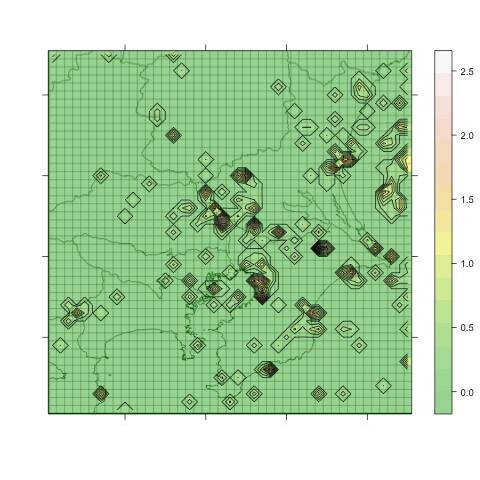
\includegraphics[scale=0.4]{media2010.jpg}
\caption{ GAModel model for the year of 2010.}
\label{modeloGAModel}
\end{figure}

\begin{figure}[H]
\centering
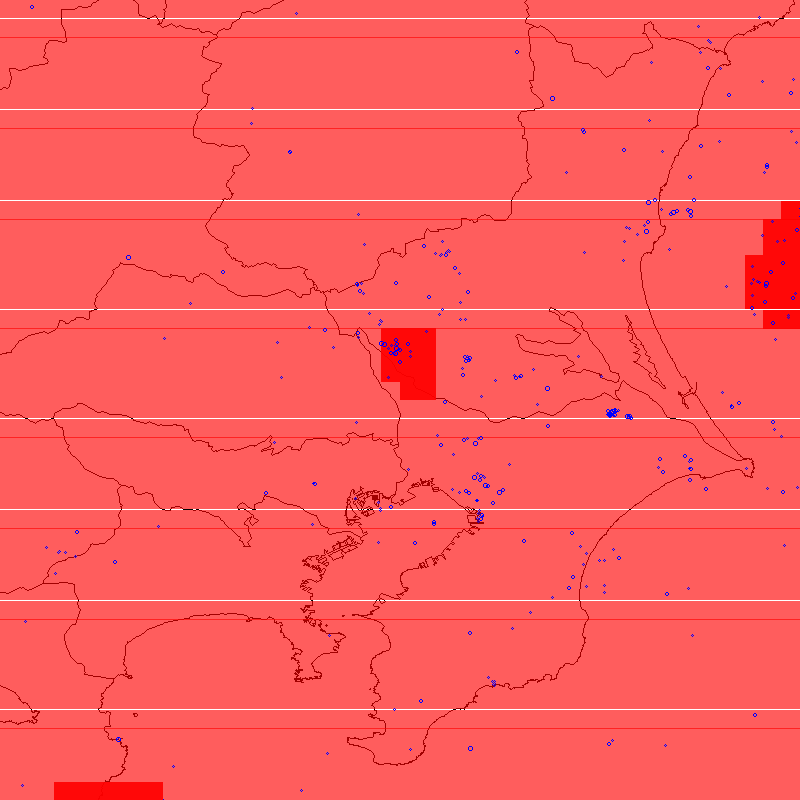
\includegraphics[scale=0.22]{kanto10_RI.png}
\caption{RI model for the year of 2010. Figure from~\cite{ecta14}.}
\label{modeloRI}
\end{figure}

\begin{figure}[H]
\centering
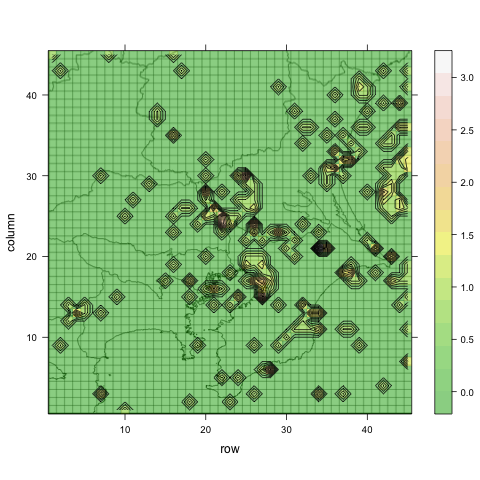
\includegraphics[scale=0.4]{matriz2010_real.png}
\caption{Earthquake occurances for the year of 2010}
\label{realData}
\end{figure}



\section{GAModel X RI Algorithm}
We compared the method proposed, ReducedGAModel,~\ref{ReducedGAModel}, with the non-variated method, GAModel~\ref{GAModel}, and with the Relative Intensity Algorithm,~\ref{ri}, using its log-likelihood values. The values are comparece via Student’s t-test, so we could understand the if there is any statistic significant difference between the methods. The data used was JMA catalog. 


\subsection{Hypothesis}
There are 3 tests hypothesis for this experiment that we want to analyse. 

The first is if the mean values of the log-likelihood for the ReducedGA are equal to the RI values.
$$\begin{cases} H_0: \mu = RI log-likelihood value&\\H_1: \mu != RI log-likelihood value\end{cases}$$

The second is if the mean values of the log-likelihood for the ReducedGA are equal to the GAModel values.
$$\begin{cases} H_0: \mu = GAModel log-likelihood value&\\H_1: \mu != GAModel log-likelihood value\end{cases}$$

And the last hypotheses is if the mean values of the log-likelihood for the GAModel are equal to the RI values.
$$\begin{cases} H_0: \mu = RI log-likelihood value&\\H_1: \mu != RI log-likelihood_value\end{cases}$$

\subsection{Results}

The results of the experiments are in the Table~\ref{gaxriTable} and in the box-plots Figure~\ref{boxPlot2007} and Figure~\ref{boxPlot2009}. The column labeled Random shows the result of the RandomModel, and the idea is the same for the ones labeled GAModel and RI. The ``p-value'' shows the significance value of the {\it Student's t-test} for the null hypothesis `` The mean of the log-likelihood values is greater that the values for RI''.\\

As expected, the RandomModel has lower values than the GAModel. When compared with the RI, the results show that the GAModel is competitive with the RI and that it is promising to use GA to generate earthquake forecasts.\\

\begin{table*}[!ht]
	\begin{center}
		\begin{tabular}{|l|l|c|cc|c|}
			\hline
			\multicolumn{1}{|c|}{Scenario} & \multicolumn{5}{|c|}{Log Likelihood} \\
			\hline
			\multicolumn{1}{|c|}{Year} & \multicolumn{1}{|c|}{Random} & \multicolumn{1}{|c|}{RI} & \multicolumn{2}{c}{GAModel} & \multicolumn{1}{|c|}{p-value} \\    
			%    Ano & Random & RI & GAModel & p-value\\
			\hline
			2000 &-2413.89 &-2124.44 &\raggedright  -2094.05 &\raggedleft (8.80) & 0.01\\%better
			2001 &-2418.14 &-2103.19 &\raggedright  -2101.65 &\raggedleft  (69.49) & 0.57\\%equal
			2002 &-2385.04 &-2094.43 &\raggedright  -2100.01 &\raggedleft (72.62) & 0.07\\%equal
			2003 &-2401.00 &-2104.65 &\raggedright  -2100.76 &\raggedleft (156) & 0.35\\%equal
			2004 &-2421.92 &-2101.92 &\raggedright  -2098.30 &\raggedleft (55.28) & 0.16\\%equal
			2005 &-2643.38 &-2248.40 &\raggedright  -2114.00 &\raggedleft (779) & 0.01\\%better
			2006 &-2616.50 &-2226.93 &\raggedright  -2115.6 &\raggedleft (633) & 0.01\\%better
			2007 &-2451.68 &-2109.13 &\raggedright  -2122.03 &\raggedleft (615) &  0.13\\%equal
			2008 &-2433.23 &-2112.92 &\raggedright  -4435.34 &\raggedleft (657) & 0.14\\%equal
			2009 &-2884.74 &-2438.10 &\raggedright  -2113.1 &\raggedleft (814) & 0.01\\%better
			2010 &-2418.18 &-2114.60 &\raggedright -2112.07 &\raggedleft (843) & 0.79\\%equal
			\hline
		\end{tabular}
	\end{center}
	\caption{Experiments result.}
	\label{gaxriTable}
\end{table*}

\begin{figure}[H]
	\centering
	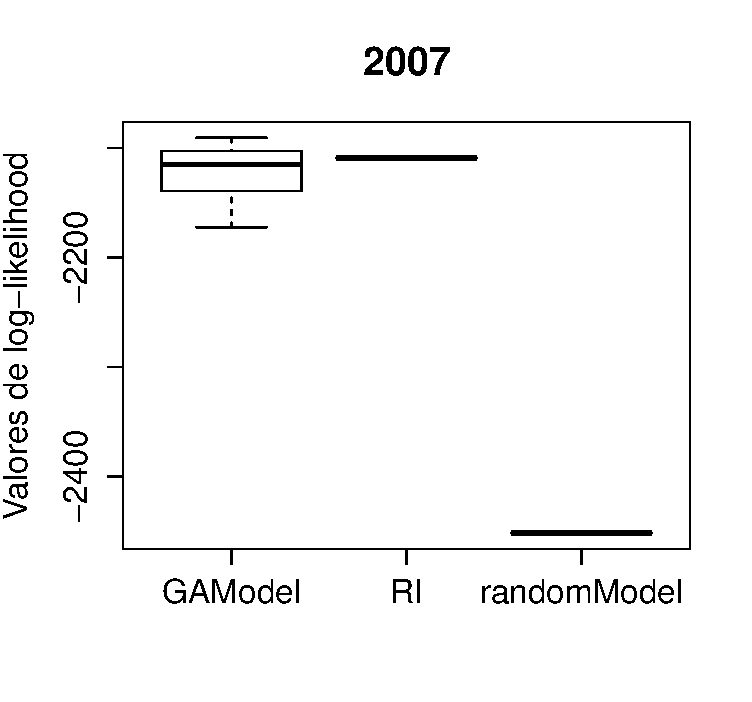
\includegraphics[scale=0.45]{boxPlot2007.pdf}
	\caption{Box-plot of the values obtained by the models for the year 2007.}
	\label{boxPlot2007}
\end{figure}

\begin{figure}[H]
	\centering
	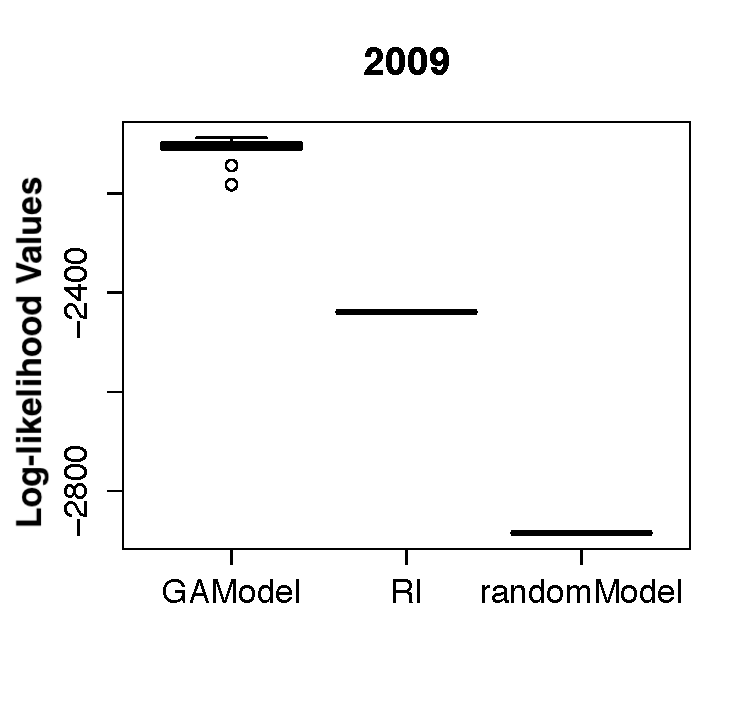
\includegraphics[scale=0.45]{boxPlot2009.pdf}
	\caption{Box-plot of the values obtained by the models for the year 2009.}
	\label{boxPlot2009}
\end{figure}


\section{All Models Experiments}
\subsection{A Brief Recapitulation of the Models}

Based on our promissing results and because we aim to improve them, we developed the ReducedGAModel. It a simplified version of the GAModel. We want to compare the behavior of this new method against the GAModel method.\\

We also wanted to explore how adding domain knowledge would improve the avarage performance of the GAModel or the ReducedGAMOdel. They are versions of GAModel/ReducedGAModel combined with emperical laws.\\ 

\subsection{The Catalogs}

The data used was JMA catalog and a version of a cluster catalog.\\ 
(JMA X métodoJanelaJMA=>clustered). How do I explain this? The EXPLANATION SHOULD BE IN THE FORMER CHAPTER
here is just a recap
\subsection{The Experiment}
For this new experiment, we used even more scenarios (space/time regions) than the ones. Each scenario contains the earthquakes for the regions of Kanto, Kansai, Touhoku and East Japan for a given year (2005-2010). We wanted to explore if there exists any influence in the performance of the models that are caused by the depth of an earthquake. So, the scenarios are also composed by introducing a 3 groups depths thresholds. They are: of earthquakes with depth smaller than 25km, or between 0km and 60km or even between 0km and 100km.\\

These method are stochastic method and hence are variations of the GAModel, we decided to maintain the number of repetitions without redoing a Power Test.\\

\subsection{ANOVA test and HSD Tukey}

The goal here is to find if there is any variation between the methods and which are the most influencial variables. For achieve that, we will use the ANOVA Test.\\

In the ANOVA test, if a variable is out of the 5\% confidence interval, with P < 0.05 it means that there exists a statistical significant different for that variable.\\

There are some tests hypothesis for this experiment that we want to analyse. They all can be generalized as follows:\\

$$\begin{cases} H_0: \text{The population means are equal populacionais são iguais.} &\\
H_1: \text{The population means are different.}&\\
\end{cases}$$\\

Then we apply a post hoc test, the HSD Tukey test, on the results obtained from the ANOVA test to specify which groups differ. \\

\subsection{Results}
A one-way between subjects ANOVA was conducted to compare the effects of the models, the depths, the years and regions on the log-likelihood value. In this study there are 6 options for model: lista, gaModel, hybridgaModel, hybridlist, gaModelCluster and listaCluster. Based on the results of the test, there was a not a significant effect of the depths or years variables. For both cases at the we obtaind p>0.05 level for the depths condition [F(2) = 2.072, p = 0.126] and we also obtained p>0.05 for the years condition  [F(5) = 0.050, p = 0.999]. There was a significant effect of the models condition (p>0.05 [F(5) = 9699.690, p<2e-16]) and regions condition (p>0.05 [F(3) = 764.220, p<2e-16]). Therefore, we conduct a new anova test, with only the last two variables to verify the influence of those conditions more accurately. The results only changed a little, maintaining the significant effect of both conditions, p>0.05 [F(5) = 9705.6, p<2e-16] and p>0.05 [F(3) = 764.7, p <2e-16], respectively.\\

The results of the experiments are in the Table~\ref{anovatest}. 

The column labeled Random shows the result of the RandomModel, and the idea the is same for the ones labeled GAModel and RI.
 means of several groups are equal,e t-test to more than two groups.
 The ``p-value'' shows significance value of the {\it Student's t-test} for null hypothesis `` The mean of the log-likelihood values is greater that the values for RI''.\\

\begin{table*}[!ht]
	\centering
	\begin{tabular}{|l|l|l|l|l|l|}
		\hline
		{Variable} & {Degrees of Freedom} & {Sum Sq}    & {Mean Sq}   & {F Value} & {Pr(\textgreater F)} \\
		\hline
		Model    & 31424058           & 6284812   & 6284812   & 255.0   & \textless2e-16     \\
		\hline
		Depth    & 2                  & 16077491  & 8038746   & 326.2   & \textless2e-16     \\
		\hline
		Year     & 5                  & 57908014  & 11581603  & 470.0   & \textless2e-16     \\
		\hline
		Region   & 3                  & 878253346 & 292751115 & 11879.4 & \textless2e-16\\    
		\hline
	\end{tabular}
	\caption{ANOVA test results.}
	\label{anovatest}
\end{table*}

Because we found statistically significant result, we applied a Post hoc comparisons using the Tukey HSD test. It compared each condition with all others. For example, it compares the values from the gaModel with the gaModelClustered, see~\ref{modelANOVA}. It indicated that the gaModelCluster and ReducedGAModelCluster, when comparared with all other models, achieve greater log-likelihood values. Furthermore, we noticed that the depths conditions show a greater influence when the depth in smaller or equal to 25 km, see Figure~\ref{depthsANOVA}\\

\begin{figure}[H]
	\centering
	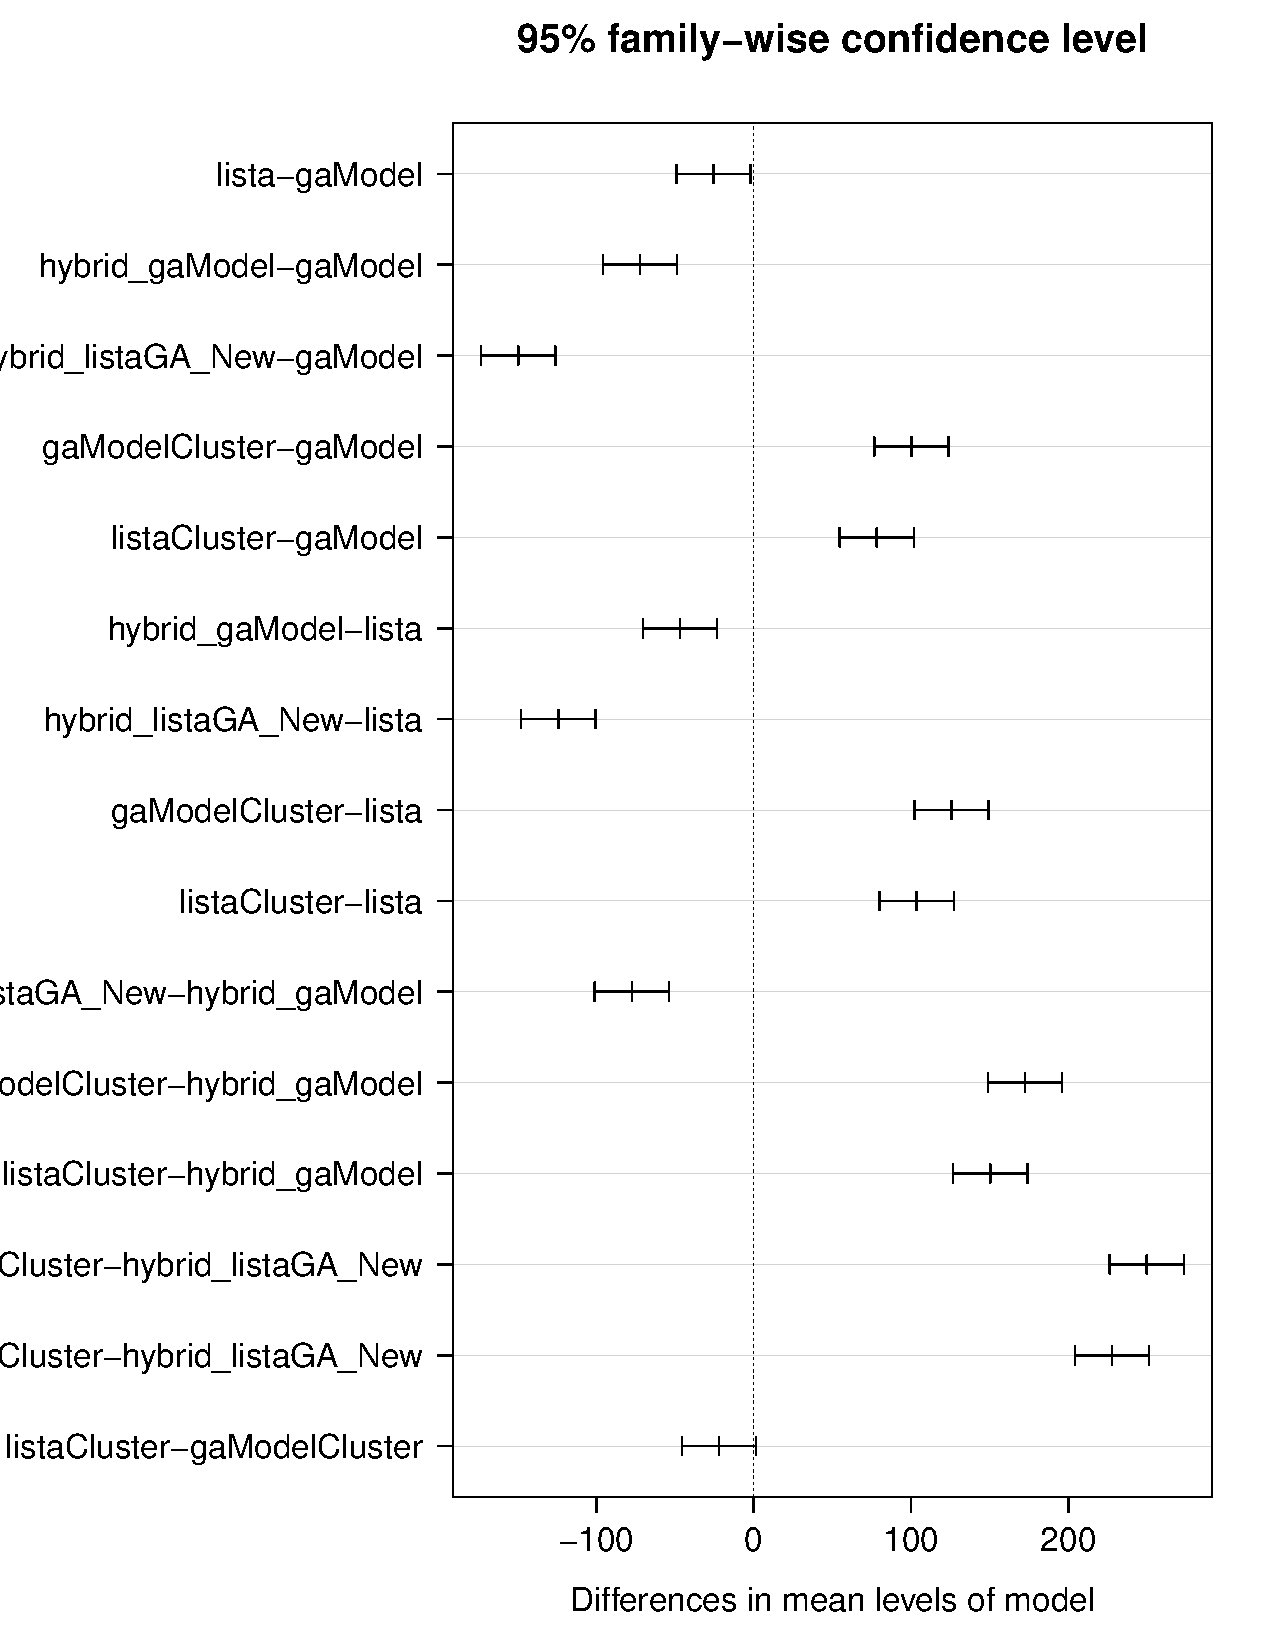
\includegraphics[scale=0.45]{modelANOVA.pdf}
	\caption{.}
	\label{modelANOVA}
\end{figure}

\begin{figure}[H]
	\centering
	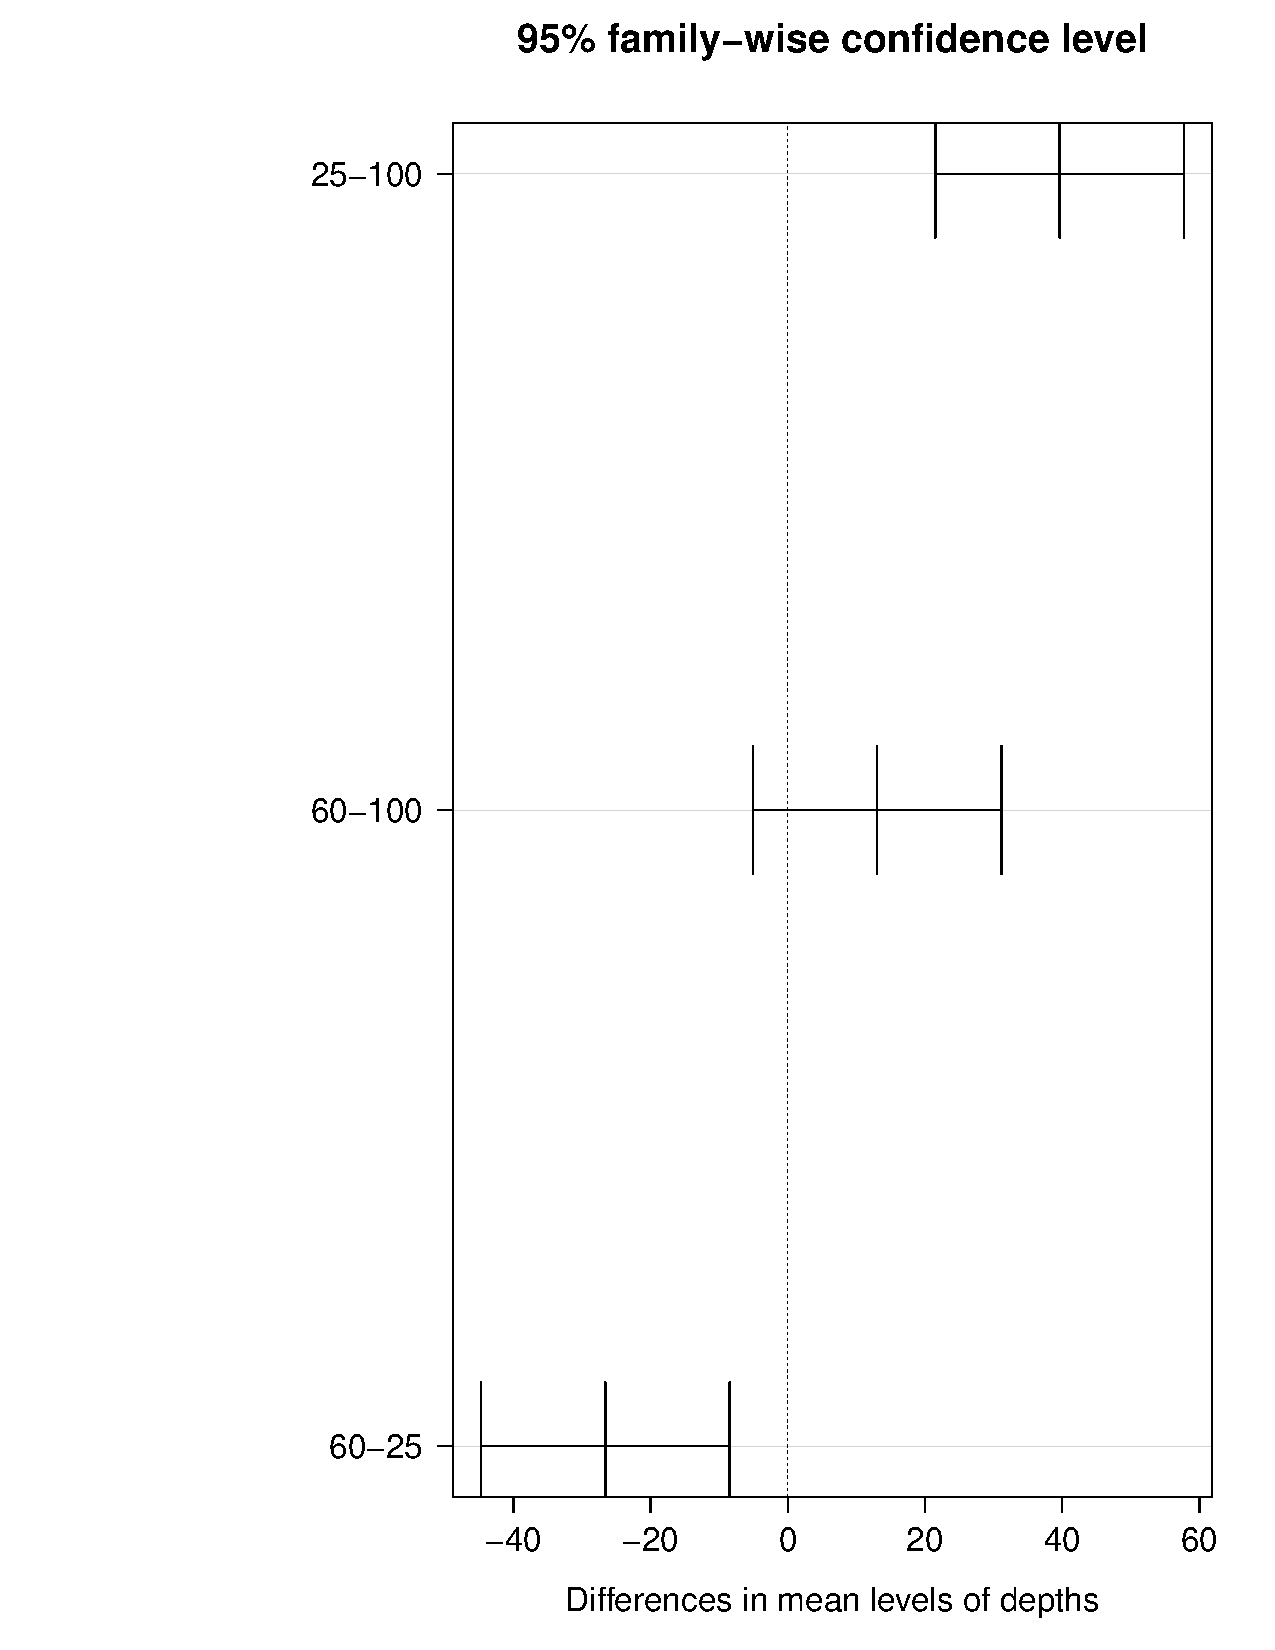
\includegraphics[scale=0.45]{depthsClusterANOVA.pdf}
	\caption{.}
	\label{depthsANOVA}
\end{figure}

When comparing the models from the ReducedGAModel and from the gaModel against themselves, with or without using clustering catalogs, we found that there is no statistically significant result between the methods. That implies it can be considered that the methods are obtain statistically equal results.\\

Therefore, based on the result of HSD test, we performed a new AVOVA test, considering only the gaModelClustered and the listaClustered. That was meant not only to verify the previous results but also to certify if the depth influence is preserved.\\

\begin{table*}[!ht]
	\centering
	\begin{tabular}{|l|l|l|l|l|l|}
		\hline
		{Variable} & {Degrees of Freedom} & {Sum Sq}    & {Mean Sq}   & {F Value} & {Pr(\textgreater F)} \\
		\hline
		Model    & 1           & 174862   & 174862   & 12.22   & \textless0.000488     \\
		\hline
		
		Depth    & 2                  & 391370  & 195685   & 13.67   & \textless1.32e-06     \\
		\hline
		Year     & 5                  & 18810831  & 3762166  & 262.82   & \textless2e-16     \\
		\hline
		Region   & 3                  & 249741769 & 83247256 & 5815.53 & \textless2e-16\\    
		\hline
	\end{tabular}
	\caption{ANOVA test results.}
	\label{anovatest}
\end{table*}


Taken together, these results suggest that the using cluster and depth smaller or equal to 25km, see Figure~\ref{depthsClusterANOVA} showed the best results.\\

\begin{figure}[H]
	\centering
	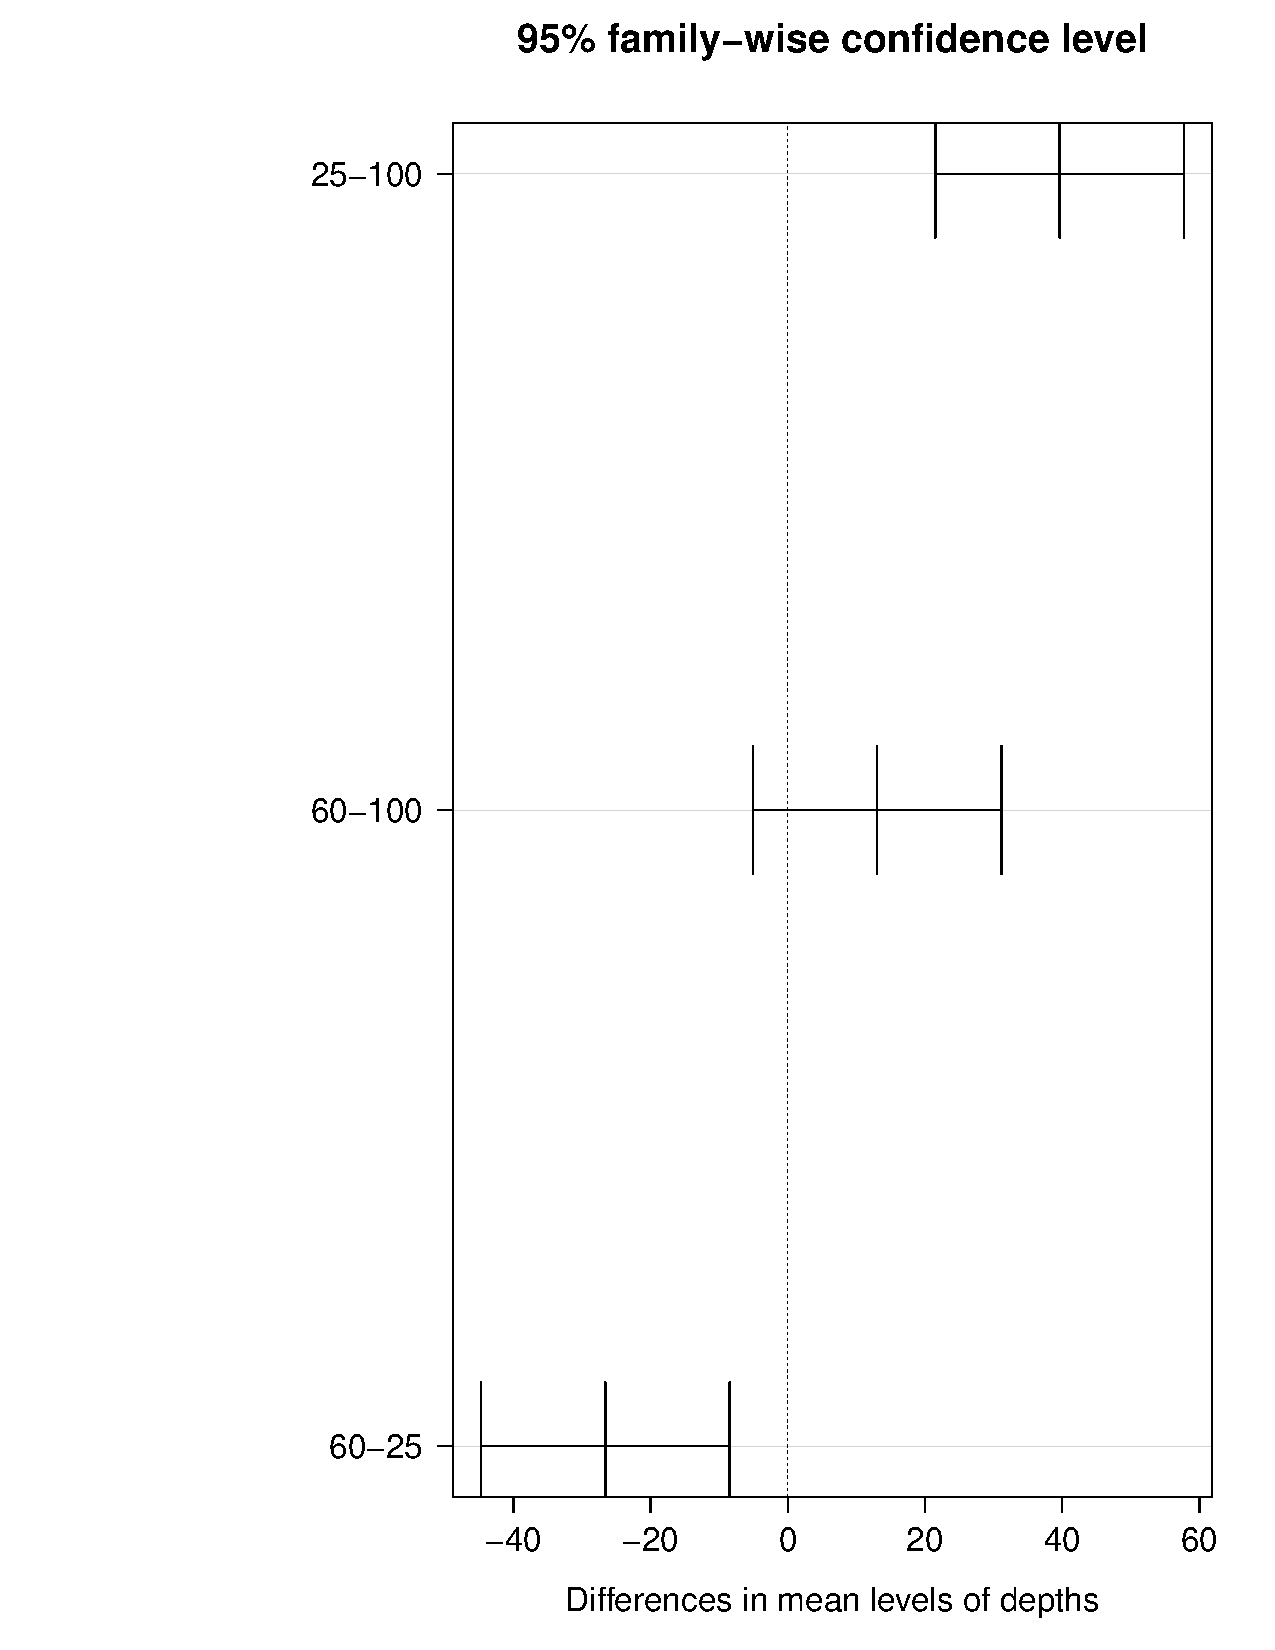
\includegraphics[scale=0.45]{depthsClusterANOVA.pdf}
	\caption{.}
	\label{depthsClusterANOVA}
\end{figure}

\section{Paired Design}

To further explore the only the variations from the models on the regions, disconsidering any other variable, we applied an paired Student’s t-test. 
 tem que fazer isso pra kanto, kansai, touhoku e EastJapan?
%TODO: tem que fazer isso pra kanto, kansai, touhoku e EastJapan?
\begin{table*}[!ht]
	\begin{center}
		\begin{tabular}{|l|l|c|cc|c|}
			\hline
			\multicolumn{1}{|c|}{Scenario} & \multicolumn{5}{|c|}{Log Likelihood} \\
			\hline
			\multicolumn{1}{|c|}{Year} & \multicolumn{1}{|c|}{Random} & \multicolumn{1}{|c|}{RI} & \multicolumn{2}{c}{GAModel} & \multicolumn{1}{|c|}{p-value} \\    
			%    Ano & Random & RI & GAModel & p-value\\
			\hline
			2000 &-2413.89 &-2124.44 &\raggedright  -2094.05 &\raggedleft (8.80) & 0.01\\%better
			2001 &-2418.14 &-2103.19 &\raggedright  -2101.65 &\raggedleft  (69.49) & 0.57\\%equal
			2002 &-2385.04 &-2094.43 &\raggedright  -2100.01 &\raggedleft (72.62) & 0.07\\%equal
			2003 &-2401.00 &-2104.65 &\raggedright  -2100.76 &\raggedleft (156) & 0.35\\%equal
			2004 &-2421.92 &-2101.92 &\raggedright  -2098.30 &\raggedleft (55.28) & 0.16\\%equal
			2005 &-2643.38 &-2248.40 &\raggedright  -2114.00 &\raggedleft (779) & 0.01\\%better
			2006 &-2616.50 &-2226.93 &\raggedright  -2115.6 &\raggedleft (633) & 0.01\\%better
			2007 &-2451.68 &-2109.13 &\raggedright  -2122.03 &\raggedleft (615) &  0.13\\%equal
			2008 &-2433.23 &-2112.92 &\raggedright  -4435.34 &\raggedleft (657) & 0.14\\%equal
			2009 &-2884.74 &-2438.10 &\raggedright  -2113.1 &\raggedleft (814) & 0.01\\%better
			2010 &-2418.18 &-2114.60 &\raggedright -2112.07 &\raggedleft (843) & 0.79\\%equal
			\hline
		\end{tabular}
	\end{center}
	\caption{Experiments result.}
	\label{gaxriTable}
\end{table*}

